\documentclass[10pt,a4paper]{article}
\usepackage[utf8]{inputenc}
\usepackage{amsmath}
\usepackage{amsfonts}
\usepackage{amssymb}
\usepackage{geometry}
\usepackage{verbatim}
\usepackage{enumerate}
\usepackage{fancyvrb}
\usepackage{graphicx}
\usepackage{tikz}
\usepackage{upgreek}
\usepackage{hyperref}

\usetikzlibrary{positioning}
\usetikzlibrary{shapes,snakes}
\usepackage[english]{babel}

\geometry{legalpaper, margin=1.5in}

\author{William Schultz}
\begin{document}
\title{Jazz Stuff}
\author{William Schultz}
\maketitle

\section{Chord Progressions}
\begin{itemize}
    \item Dominant cadence: V-I
    \item Two-five-one: ii-V-I
\end{itemize}

\section{Dominant Substitutions}

In any progression that resolves with a dominant cadence (e.g. ii-V-I), we can replace the V chord with an alternate substitution. A set of common substitutions can be thought of as being taken from the tones of diminished 7 V chord. For example, in Cmaj, consider the tones of the diminished chord for the V, Gdim7 (G B$\flat$ D$\flat$ E), and use their dominant 7 chords as substitutions for the V chord. This gives us the following substitutions: 
\begin{itemize}
    \item G7 (Dominant)
    \item B$\flat$7 ($\flat\text{VII}^7$, ``flat 7 7")
    \item D$\flat$7 (Tritone substitution)
    \item E7 (less common)
\end{itemize}
Can also get to the the above dominant substitutions via their respective ii chords e.g. $$A \flat m7 - D \flat 7$$ Note that such a 2-5-1 progression on the $\flat\text{VII}^7$ is also referred to as the ``backdoor'' 2-5 progression. For example, in C major this progression is Fm7 - B$\flat$7 - C.

\subsubsection*{Relationship to Altered Dominants}

Note that the tritone substitution has the same key chord tones as the normal dominant, the 3rd and 7th i.e. a $D\flat 7$ contains both F and B, the 3rd and 7th of G7. So, the tritone is in some sense effective as a dominant resolution for similar reasons to the standard dominant chord. But, it can also be thought of as containing tones of an altered dominant chord. This is the same for the $\flat\text{VII}^7$ substitution. Specifically:
\begin{itemize}
    \item Dominant: 1 3 5 7
    \item $\flat\text{VII}^7$: $\sharp$9 5 7 $\flat$9 
    \item Tritone sub: $\sharp$11 7 $\flat$9 3
\end{itemize}
That is, tritone sub can be viewed as nearly functionally identical to a $G7 \flat 9 \sharp 11$ in terms of chord tones, also with just chromatic bass movement ($D \flat$ to $C$ instead of $G$ to $C$.)

See also worksheet below on reharmonization:
\begin{center}
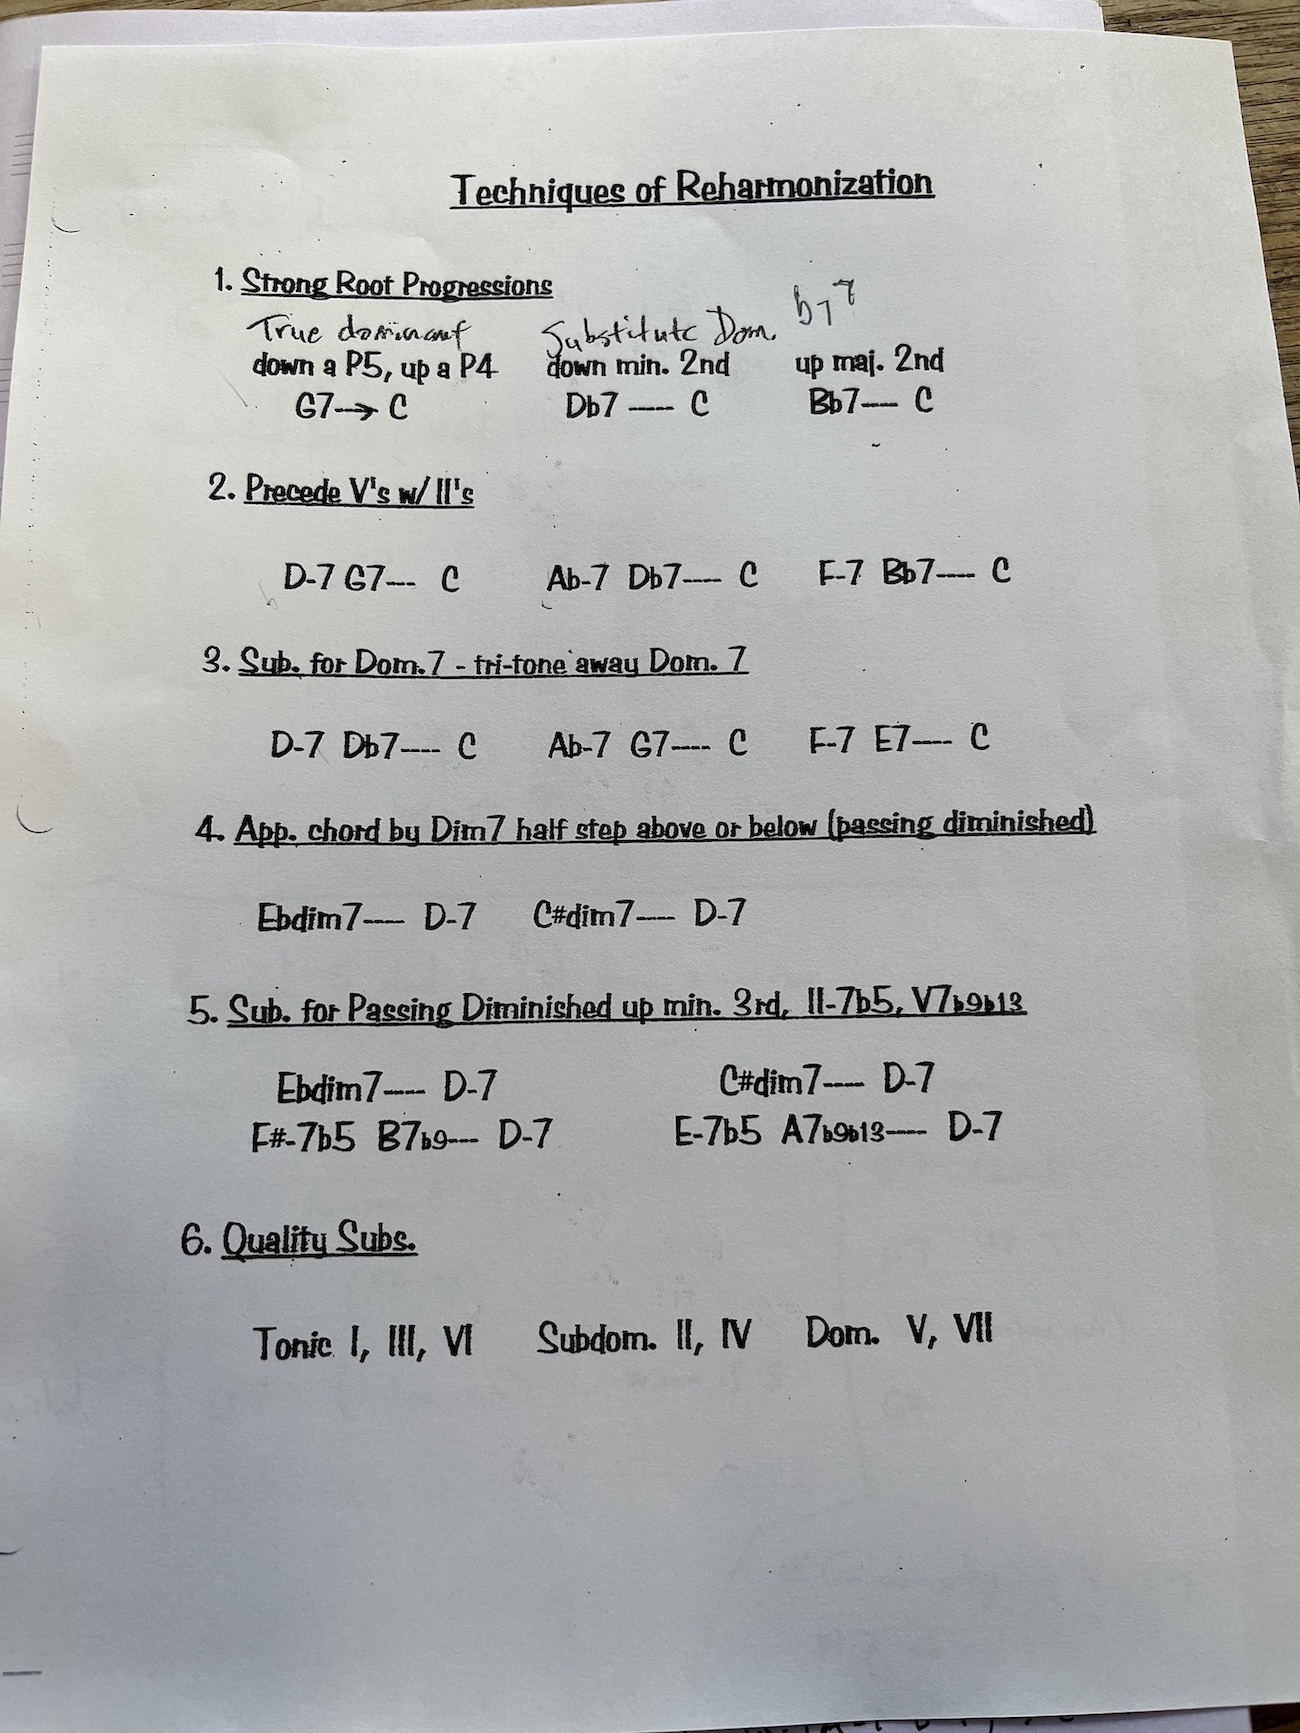
\includegraphics[scale=0.15]{reharmonization_techniques.jpg}
\end{center}

\section{Tunes (w/ keys)}

\begin{enumerate}
    \item Autumn Leaves (B$\flat$, G)
    \item There Will Never Be Another You (E$\flat$, B$\flat$) (\textit{Form}: ABAC)
    \item Misty (E$\flat$)
    \item All the Things You Are
    \item There Is No Greater Love (B$\flat$) (\textit{Form}: AABA)
    \item These Foolish Things (E$\flat$)
    \item Blue Bossa
    \item Blue Monk
    \item Night In Tunisia
    \item All of Me
    \item Solar
    \item Have You Met Miss Jones
    \item Someday My Prince Will Come

\end{enumerate}

\end{document}